% This is text associated with the open textbook "Open Electromagnetics"
% See immediately below for author, date
% This work is licensed under the Creative Commons Attribution-ShareAlike 4.0 International License. (CC BY-SA 4.0) 
% To view a copy of the license, visit http://creativecommons.org/licenses/by-sa/4.0/

%ORB TITLE Electric Field Due to an Infinite Line Charge using Gauss' Law
%ORB AUTHOR 0        # S.W. Ellingson, Virginia Tech (ellingson@vt.edu)
%ORB DATE 20180803   # yyyymmdd
%ORB ABSTRACT Electric Field Due to an Infinite Line Charge using Gauss' Law

\label{m0149_E_due_to_Inf_Line_Charge} % <-- Must match name of this file and module directory name.  Don't mess with this!
\index{Gauss' law!electric field}

Section~\ref{m0014_Gauss_Law_Integral_Form} explains one application of Gauss' Law, which is to find the electric field due to a charged particle.
In this section, we present another application -- the electric field due to an infinite line of charge.
The result serves as a useful ``building block'' in a number of other problems, including determination of the capacitance of coaxial cable (Section~\ref{m0113_Capacitance_of_Coaxial_Line}).
Although this problem can be solved using the ``direct'' approach described in Section~\ref{m0104_E_due_to_a_Continuous_Distribution_of_Charge} (and it is an excellent exercise to do so), the Gauss' Law approach demonstrated here turns out to be relatively simple.

%ORB EXAMPLE
~\\ \begin{example} 
\begin{mdframed}[backgroundcolor=brown!20,linecolor=brown!20]\raggedright
Electric field associated with an infinite line charge, using Gauss' Law.
\index{charge density!line} 
\\~\\
Use Gauss' Law to determine the electric field intensity due to an infinite line of charge along the $z$ axis, having charge density $\rho_l$ (units of C/m), as shown in Figure~\ref{m0149_fGLLS}.

{\bf Solution.}
Gauss' Law requires integration over a surface that encloses the charge.
So, our first problem is to determine a suitable surface.
A cylinder of radius $a$ that is concentric with the $z$ axis, as shown in Figure~\ref{m0149_fGLLS}, is maximally symmetric with the charge distribution and so is likely to yield the simplest possible analysis.
At first glance, it seems that we may have a problem since the charge extends to infinity in the $+z$ and $-z$ directions, so it's not clear how to enclose all of the charge. 
Let's suppress that concern for a moment and simply choose a cylinder of finite length $l$.
In principle, we can solve the problem first for this cylinder of finite size, which contains only a fraction of the charge, and then later let $l\to\infty$ to capture the rest of the charge.
(In fact, we'll find when the time comes it will not be necessary to do that, but we shall prepare for it anyway.)

Here's Gauss' Law:
%
\begin{equation}
\oint_{\mathcal S} {\bf D}\cdot d{\bf s} = Q_{encl}
\label{m0149_eGL}
\end{equation}
%
where 
${\bf D}$ is the electric flux density $\epsilon{\bf E}$,
${\mathcal S}$ is a closed surface with outward-facing differential surface normal $d{\bf s}$, and
$Q_{encl}$ is the enclosed charge.

The first order of business is to constrain the form of ${\bf D}$ using a symmetry argument, 
\index{symmetry}
as follows.
Consider the field of a point charge $q$ at the origin (Section~\ref{m0014_Gauss_Law_Integral_Form}): 
%
\begin{equation}   
{\bf D}  = \hat{\bf r}\frac{q}{4\pi r^2}
\end{equation}
%
We can ``assemble'' an infinite line of charge by adding particles in pairs.
One pair is added at a time, with one particle on the $+z$ axis and the other on the $-z$ axis, with each located an equal distance from the origin. 
We continue to add particle pairs in this manner until the resulting charge extends continuously to infinity in both directions.
The principle of superposition indicates that the resulting field will be the sum of the fields of the particles (Section~\ref{m0103_E_due_to_Point_Charges}).
Thus, we see that ${\bf D}$ cannot have any component in the $\hat{\bf \phi}$ direction because none of the fields of the constituent particles have a component in that direction.
Similarly, we see that the magnitude of ${\bf D}$ cannot depend on $\phi$ because none of the fields of the constituent particles depends on $\phi$ and because the charge distribution is identical (``invariant'') with rotation in $\phi$.
Also, note that for any choice of $z$ the distribution of charge above and below that plane of constant $z$ is identical; therefore, ${\bf D}$ cannot be a function of $z$ \emph{and} ${\bf D}$  cannot have any component in the $\hat{\bf z}$ direction.
Therefore, the direction of ${\bf D}$ must be radially outward; i.e., in the $\hat{\bf \rho}$ direction, as follows:
%
\begin{equation}
{\bf D} = \hat{\bf \rho}D_{\rho}(\rho)
\end{equation}

Next, we observe that $Q_{encl}$ on the right hand side of Equation~\ref{m0149_eGL} is equal to $\rho_l l$.  Thus, we obtain
%
\begin{equation}
\oint_{\mathcal S} \left[\hat{\bf \rho}D_{\rho}(\rho)\right] \cdot d{\bf s} = \rho_l l
\end{equation}
%
The cylinder $\mathcal{S}$ consists of a flat top, curved side, and flat bottom.  Expanding the above equation to reflect this, we obtain
%
\begin{flalign}
\rho_l l =&~~~ \int_{top} \left[\hat{\bf \rho}D_{\rho}(\rho)\right] \cdot \left(+\hat{\bf z}ds\right)    \nonumber \\
          &+ \int_{side} \left[\hat{\bf \rho}D_{\rho}(\rho)\right] \cdot \left(+\hat{\bf \rho}ds\right) \nonumber \\
          &+ \int_{bottom} \left[\hat{\bf \rho}D_{\rho}(\rho)\right] \cdot \left(-\hat{\bf z}ds\right)   
\end{flalign}
%
Examination of the dot products indicates that the integrals associated with the top and bottom surfaces must be zero.  
In other words, the flux through the top and bottom is zero because ${\bf D}$ is perpendicular to these surfaces.
We are left with
%
\begin{equation}
\rho_l l = \int_{side} \left[D_{\rho}(\rho)\right] ds 
\end{equation}
%
The side surface is an open cylinder of radius $\rho=a$, so $D_{\rho}(\rho)=D_{\rho}(a)$, a constant over this surface.  Thus:
%
\begin{equation}
\rho_l l = \int_{side} \left[D_{\rho}(a)\right] ds =  \left[D_{\rho}(a)\right] \int_{side} ds 
\end{equation}
%
The remaining integral is simply the area of the side surface, which is $2\pi a \cdot l$.
Solving for $D_{\rho}(a)$ we obtain
%
\begin{equation}
D_{\rho}(a) = \frac{\rho_l l}{2\pi a l} = \frac{\rho_l}{2\pi a}
\end{equation}
%
Remarkably, we see $D_{\rho}(a)$ is independent of $l$, So the concern raised in the beginning of this solution -- that we wouldn't be able to enclose all of the charge -- doesn't matter.

Completing the solution, we note the result must be the same for any value of $\rho$ (not just $\rho=a$), so
%
\begin{equation}
{\bf D} = \hat{\rho} D_{\rho}(\rho) = \hat{\rho} \frac{\rho_l}{2\pi \rho}
\end{equation}
%
and since ${\bf D}=\epsilon{\bf E}$:
%
\begin{equation}
\boxed{
{\bf E} = \hat{\rho} \frac{\rho_l}{2\pi \epsilon \rho}
}
\end{equation}
%
This completes the solution.
We have found that the electric field is directed radially away from the line charge, and decreases in magnitude in inverse proportion to distance from the line charge. 
Suggestion: Check to ensure that this solution is dimensionally correct.
\end{mdframed}
%
\begin{figure}
\begin{center}
\pdftooltip{{  % note double braces
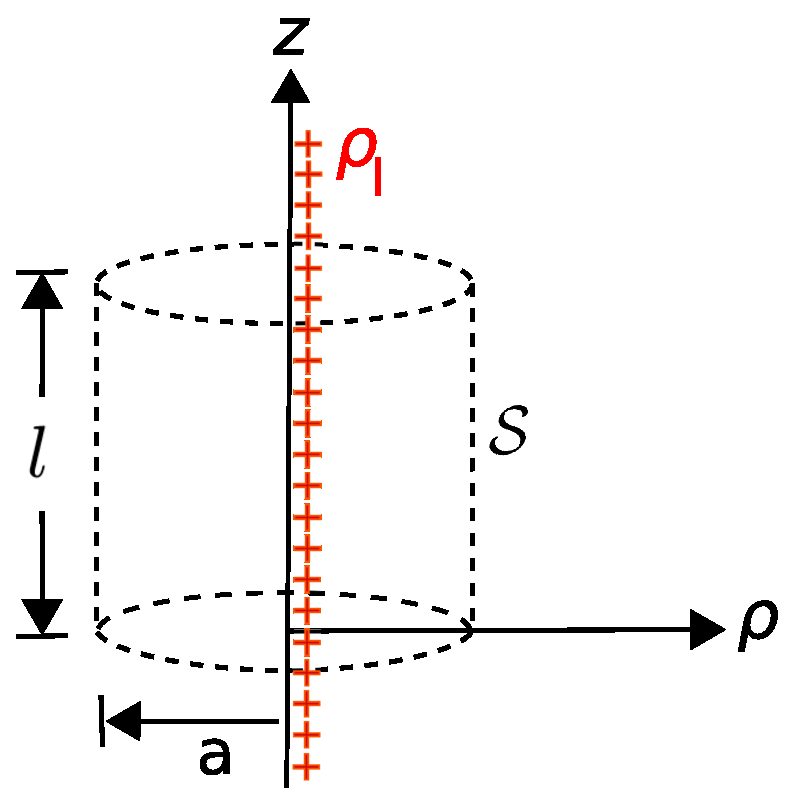
\includegraphics[width=2in]{modules/m0149_fGLLS.eps}
}}{rho and z axes are shown. A cylinder drawn with a dashed line is centered about the z axis. The lower face is positioned at the origin. Radius (a) shown from the z axis to the surface of the cylinder. Length (l) is parallel to z-axis. Positive charge is represented by orange plus signs extending to infinity in the positive and negative z direction, labeled rho sub l.}
\end{center} 
\centerline{\scriptsize 
\copyright~\hyperref[m0149_fGLLS_Credit]{K.\ Kikkeri} 
\href{https://creativecommons.org/licenses/by-sa/4.0/}{CC BY~SA 4.0} 
} 
\caption{
\label{m0149_fGLLS}
Finding the electric field of an infinite line of charge using Gauss' Law.
}
\end{figure}
\end{example}



